\documentclass{beamer}

\usepackage[orientation=portrait, size=a0, scale=1.4]{beamerposter}

% \usetheme{confposter} % Use the confposter theme supplied with this template

\usepackage[utf8]{inputenc}
\usepackage[T1]{fontenc}
\usepackage[francais]{babel}

\usepackage{graphicx}
\usepackage{subfig}
\usepackage{xcolor}
\usepackage{enumitem}

\definecolor{tagada}{RGB}{172, 42, 42}
\definecolor{tagado}{RGB}{42, 42, 172}

\setbeamertemplate{blocks}[rounded][shadow=false]

\begin{document}
    \begin{frame}[t]
        %---------------------------
        %-          TITLE          -
        %---------------------------

        \setbeamercolor{block body}{fg=black,bg=green} % Colors of the block titles
        \begin{block}{}
            \begin{columns}[t]
                \begin{column}{.1\linewidth}
                    \begin{figure}[t]
                        
\includegraphics[width=\linewidth]{rsc/logo_um.png}
                    \end{figure}
                \end{column}

                \begin{column}{.75\linewidth}
                    \begin{center}
                        {\Huge \textbf{Musée sécurisé en réalité augmentée}}
                    \end{center}

                    \begin{columns}[t]
                        \begin{column}{.5\linewidth}
                            \begin{center}
                                \textbf{Présenté par\\Théo Clayette, Thibaut Etienne, Arnaud Soulier}
                            \end{center}
                        \end{column}

                        \begin{column}{.5\linewidth}
                            \begin{center}
                                \textbf{Sous la direction de\\William Puech, Pauline Puteaux}
                            \end{center}
                        \end{column}
                    \end{columns}
                \end{column}

                \begin{column}{.1\linewidth}
                    \begin{figure}[t]
                        
\includegraphics[width=\linewidth]{rsc/logo_lirmm.png}
                    \end{figure}
                \end{column}
            \end{columns}
        \end{block}

        % \rule{\linewidth}{2mm}

        %----------------------------
        %-          POSTER          -
        %----------------------------

        \begin{columns}[t]
            %------------------------------------------
            %-          POSTER - CHIFFREMENT          -
            %------------------------------------------

            \begin{column}{.5\linewidth}
                \begin{center}
                    {\textbf{Chiffrement}}
                \end{center}

                %--------------------------------
                %-          C1 - INDEX          -
                %--------------------------------

                \setbeamercolor{block title}{fg=white,bg=blue} % Colors of the block titles
                \setbeamercolor{block body}{fg=black,bg=white} % Colors of the block titles
                \begin{block}{\centering \textbf{Index}}
                    \begin{figure}[t]
                        \begin{center}
                            \captionsetup[subfigure]{justification=centering}
                            \subfloat[Itération 1]{
                                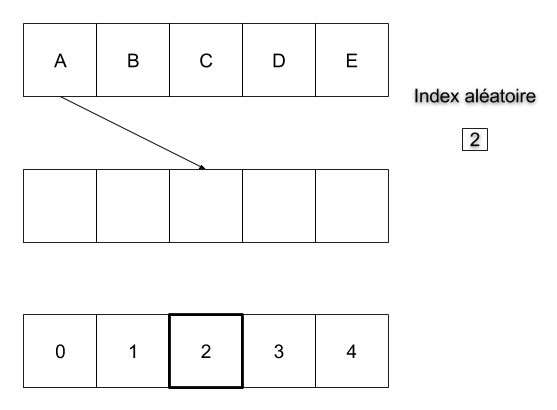
\includegraphics[width=.3\linewidth]{rsc/index1_1.png}}
                            \subfloat[Itération 2]{
                                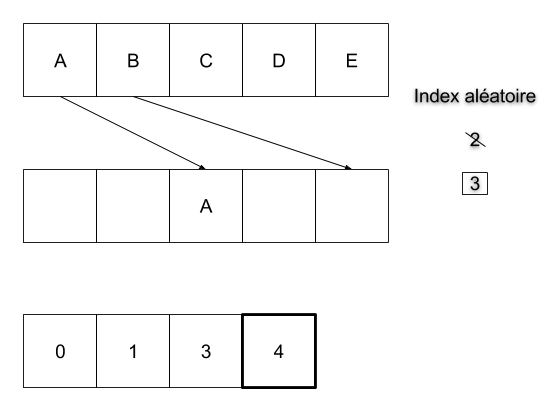
\includegraphics[width=.3\linewidth]{rsc/index1_2.png}}
                            \subfloat[Itération 3]{
                                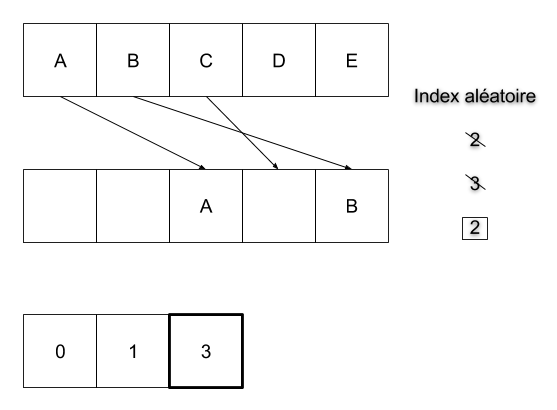
\includegraphics[width=.3\linewidth]{rsc/index1_3.png}}
                            \caption{Algorithme de chiffrement pseudo-aléatoire}
                        \end{center}
                    \end{figure}

                    Chaque itération se décompose en 4 étapes :
                    \begin{itemize}[label=-]
                        \item Tirage d'un nombre aléatoire $r$ entre 0 et la taille d'un tableau d'index.
                        \item Récupération du nouvel indice $n$ du pixels dans le tableau d'index à l'indice $r$.
                        \item Écriture du pixels dans la nouvelle case $n$ de l'image de sortie.
                        \item Suppression de la case $n$ du tableau d'index.
                    \end{itemize}
                \end{block}

                %------------------------------------
                %-          C1 - Résultats          -
                %------------------------------------

                \setbeamercolor{block title}{fg=white,bg=green} % Colors of the block titles
                \setbeamercolor{block body}{fg=black,bg=white} % Colors of the block titles
                \begin{block}{\centering \textbf{Résultats}}
                    \begin{figure}[t]
                        \begin{center}
                            \captionsetup[subfigure]{justification=centering}
                            \subfloat[Image original de 800x800 pixels]{
                                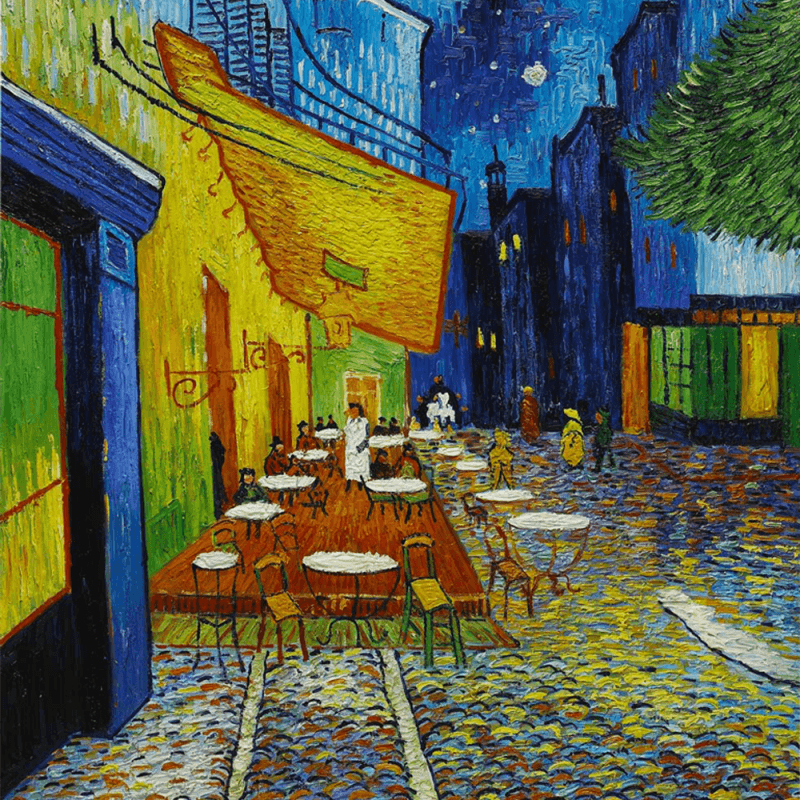
\includegraphics[width=.25\linewidth]{rsc/van_gogh.png}}
                            \hspace{.05\linewidth}
                            \subfloat[Chiffrement par 800x800 blocs de 1x1 pixels]{
                                
\includegraphics[width=.25\linewidth]{rsc/van_gogh_800_12.png}}\\
                            \subfloat[Chiffrement par 10x10 blocs de 80x80 pixels]{
                                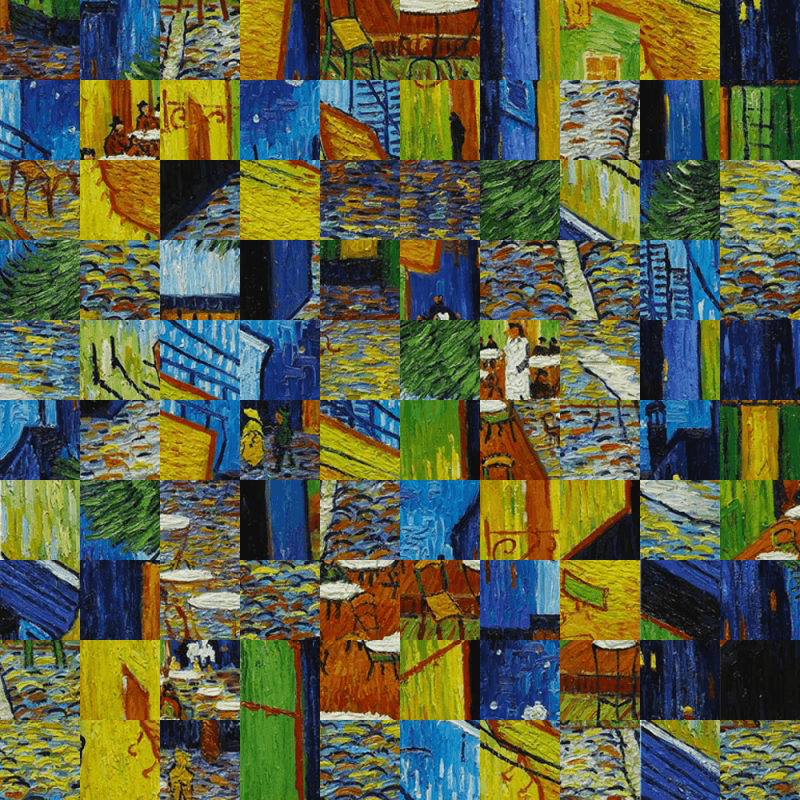
\includegraphics[width=.25\linewidth]{rsc/van_gogh_10_12.png}}
                            \hspace{.05\linewidth}
                            \subfloat[Chiffrement par 25x25 blocs de 32x32 pixels]{
                                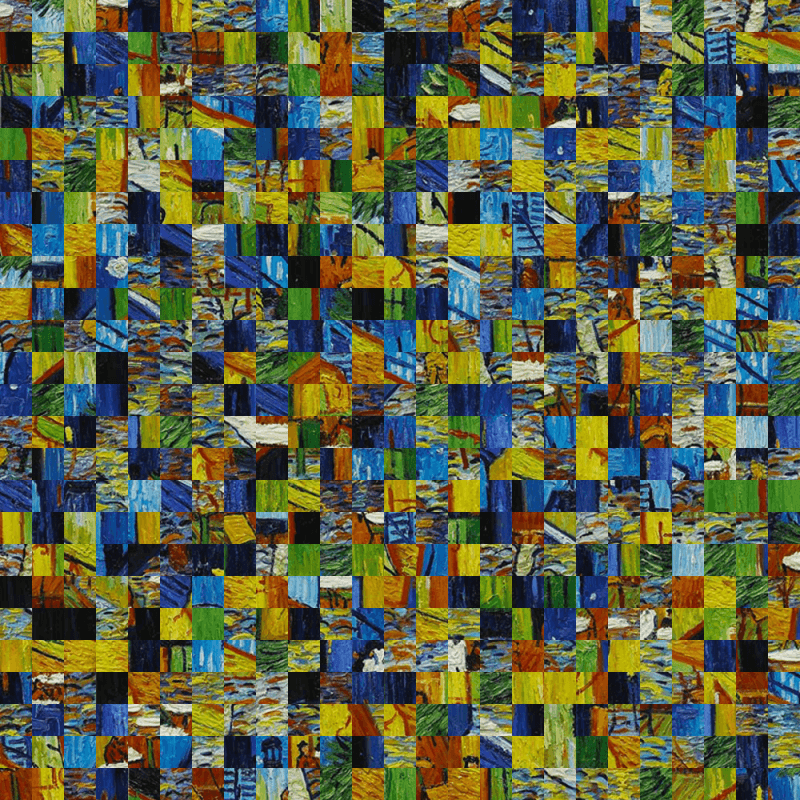
\includegraphics[width=.25\linewidth]{rsc/van_gogh_25_12.png}}
                            \hspace{.05\linewidth}
                            \subfloat[Chiffrement par 50x50 blocs de 16x16 pixels]{
                                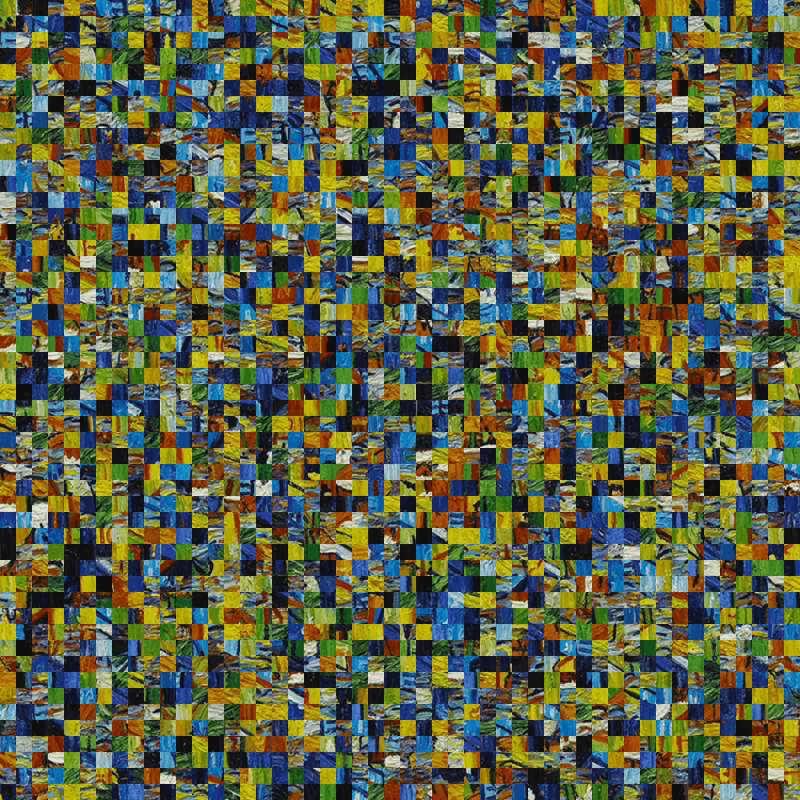
\includegraphics[width=.25\linewidth]{rsc/van_gogh_50_12.png}}\\
                            \subfloat[Chiffrement par 10x10 blocs de 80x80 pixels moyennés]{
                                
\includegraphics[width=.25\linewidth]{rsc/van_gogh_a_10_12.png}}
                            \hspace{.05\linewidth}
                            \subfloat[Chiffrement par 25x25 blocs de 32x32 pixels moyennés]{
                                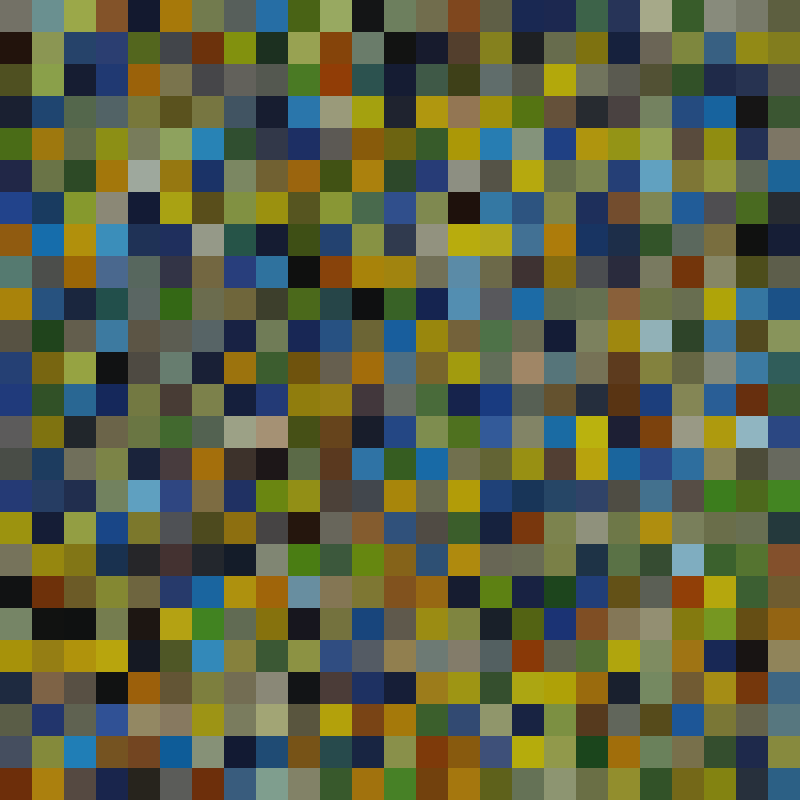
\includegraphics[width=.25\linewidth]{rsc/van_gogh_a_25_12.png}}
                            \hspace{.05\linewidth}
                            \subfloat[Chiffrement par 50x50 blocs de 16x16 pixels moyennés]{
                                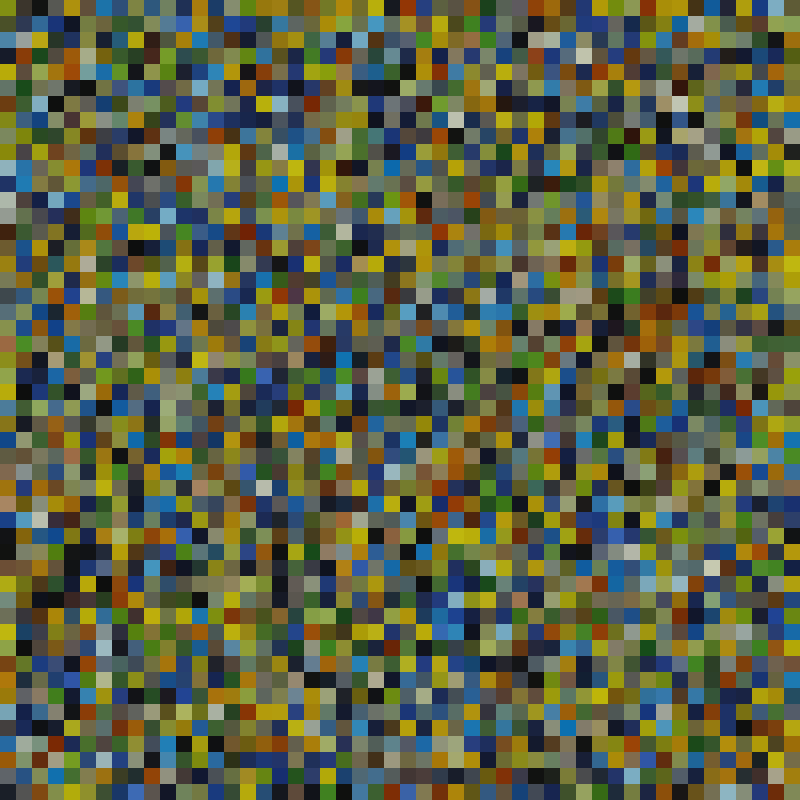
\includegraphics[width=.25\linewidth]{rsc/van_gogh_a_50_12.png}}\\
                            \caption{Chiffrement par bloc et bloc moyenné de la peinture "Térasse du café le soir" de Van Gogh}
                        \end{center}
                    \end{figure}
                \end{block}
            \end{column}

            %--------------------------------------------
            %-          POSTER - DECHIFFREMENT          -
            %--------------------------------------------

            \begin{column}{.5\linewidth}
                \begin{center}
                    {\textbf{Déhiffrement}}
                \end{center}

                %----------------------------------------
                %-          C2 - PRETRAITEMENT          -
                %----------------------------------------

                \setbeamercolor{block title}{fg=white,bg=red} % Colors of the block titles
                \setbeamercolor{block body}{fg=black,bg=white} % Colors of the block titles
                \begin{block}{\centering \textbf{Prétraitements}}
                    Traitement à effectuer sur la photo pour permettre la transformation :
                    \begin{itemize}[label=\textbullet]
                        \item Conversion en image en niveau de gris :
                        \begin{itemize}[label=$\rightarrow$]
                            \item 0.299 $\cdot$ rouge + 0.587 $\cdot$ vert + 0.114 $\cdot$ bleu.
                        \end{itemize}
                        \item Conversion en image binaire :
                        \begin{itemize}[label=$\rightarrow$]
                            \item sépare la peinture du fond pour failiter la détection des angles.
                        \end{itemize}
                        \item Détection des angles :
                        \begin{itemize}[label=$\rightarrow$]
                            \item Trouve les coordonnées des quatres angle pour les prendre comme base de l'algorithme de transformation.
                        \end{itemize}
                    \end{itemize}
                \end{block}

                %----------------------------------------
                %-          C2 - TRANFORMATION          -
                %----------------------------------------

                \setbeamercolor{block title}{fg=white,bg=blue} % Colors of the block titles
                \setbeamercolor{block body}{fg=blue,bg=white} % Colors of the block titles
                \begin{block}{\centering \textbf{Transformation}}
                    \begin{figure}[t]
                        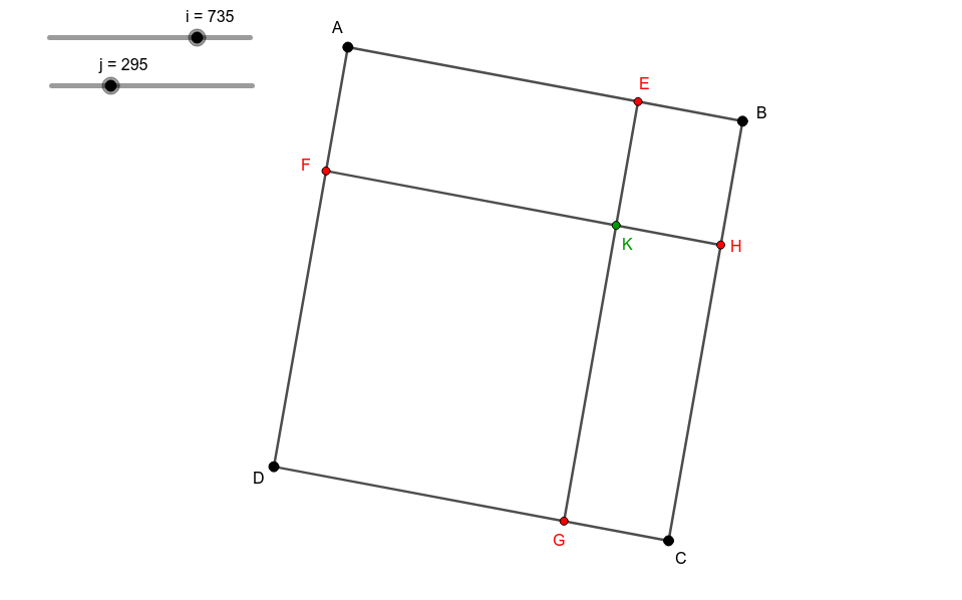
\includegraphics[width=.5\linewidth]{rsc/transform_formula.png}\\
                    \end{figure}
                \end{block}

                %------------------------------------
                %-          C2 - RESULTATS          -
                %------------------------------------

                \setbeamercolor{block title}{fg=white,bg=green} % Colors of the block titles
                \setbeamercolor{block body}{fg=black,bg=white} % Colors of the block titles
                \begin{block}{\centering \textbf{Résultats}}
                    \begin{columns}[t]
                        \begin{column}{.2\linewidth}
                            \begin{figure}[t]
                                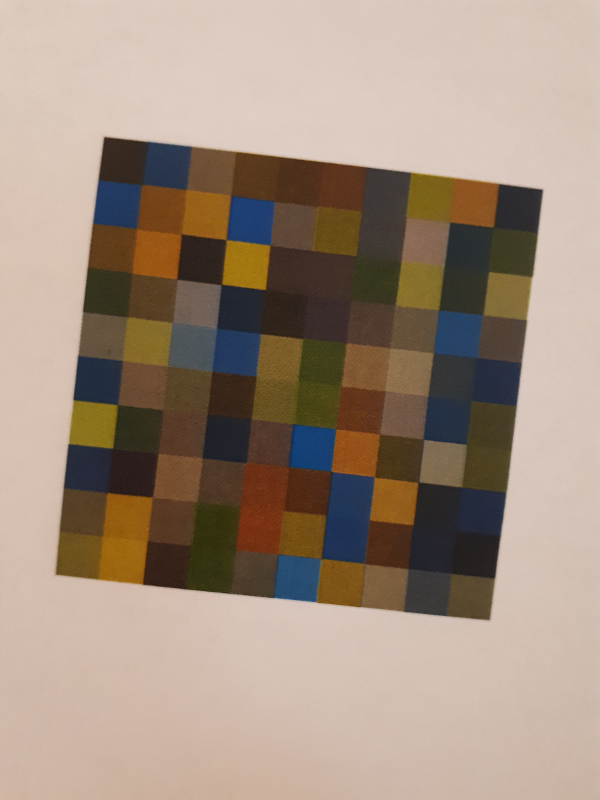
\includegraphics[width=\linewidth]{rsc/van_gogh_picture_a_10.png}\\
                            \end{figure}
                        \end{column}

                        \begin{column}{.2\linewidth}
                            \begin{figure}[t]
                                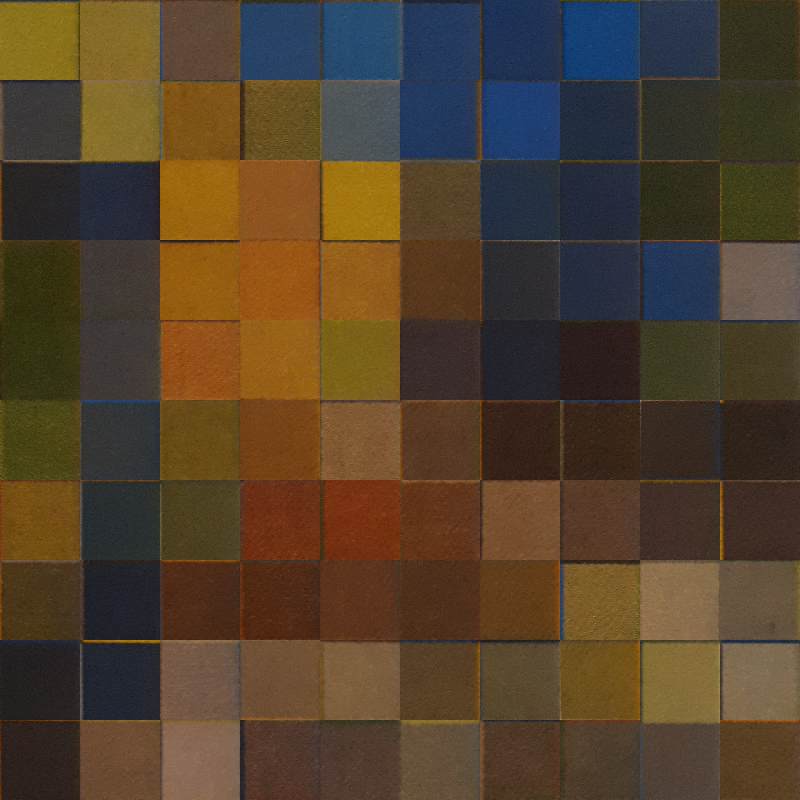
\includegraphics[width=\linewidth]{rsc/van_gogh_picture_a_10_d.png}\\
                            \end{figure}
                        \end{column}

                        \begin{column}{.005\linewidth}

                        \end{column}

                        \begin{column}{.2\linewidth}
                            \begin{figure}[t]
                                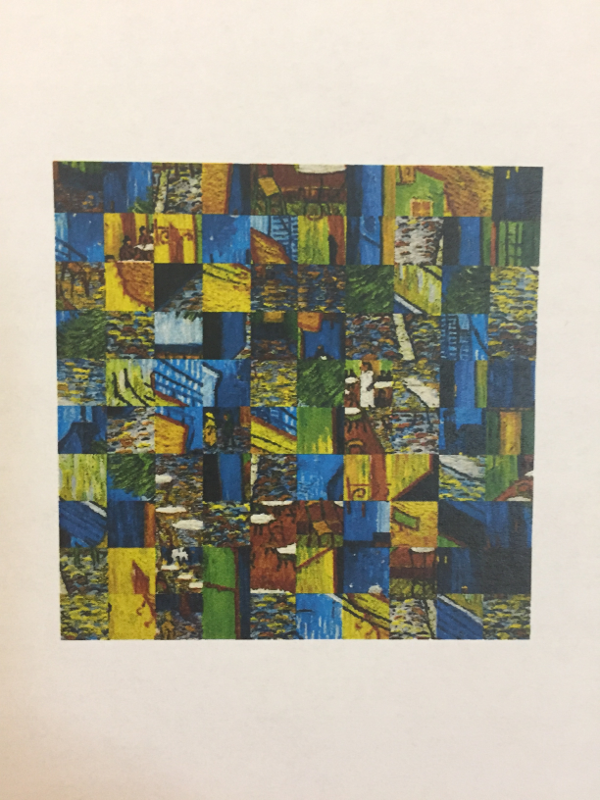
\includegraphics[width=\linewidth]{rsc/van_gogh_picture_10.png}\\
                            \end{figure}
                        \end{column}

                        \begin{column}{.2\linewidth}
                            \begin{figure}[t]
                                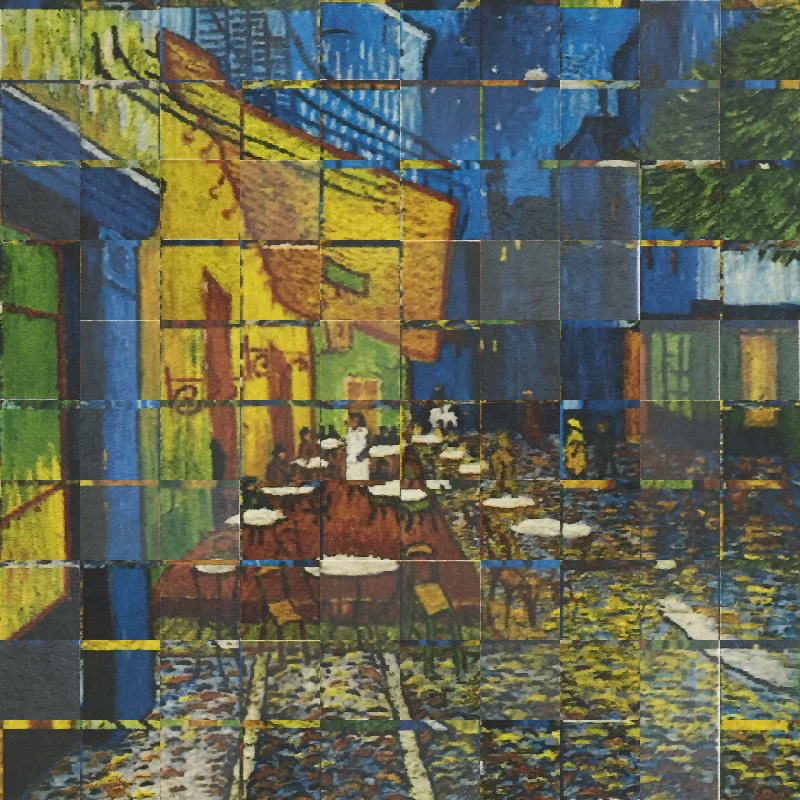
\includegraphics[width=\linewidth]{rsc/van_gogh_picture_10_d.png}\\
                            \end{figure}
                        \end{column}
                    \end{columns}

                    \begin{columns}[t]
                        \begin{column}{.5\linewidth}
                            \begin{center}
                                {\small Déchiffrement 10x10 blocs de 80x80 pixels moyennés}
                            \end{center}
                        \end{column}

                        \begin{column}{.5\linewidth}
                            \begin{center}
                                {\small Déchiffrement 10x10 blocs de 80x80 pixels}
                            \end{center}
                        \end{column}
                    \end{columns}
                \end{block}
            \end{column}
        \end{columns}

        %--------------------------------------
        %-          POSTER - QUALITE          -
        %--------------------------------------

        \begin{columns}[t]

            %-----------------------------------------
            %-          C3 - Reconnaissance          -
            %-----------------------------------------

            \begin{column}{.5\linewidth}
                \setbeamercolor{block title}{fg=white,bg=black} % Colors of the block titles
                \setbeamercolor{block body}{fg=black,bg=white} % Colors of the block titles
                \begin{block}{\centering \textbf{Ressemblance de l'image}}


                    \begin{center}
                        \begin{figure}[t]
                            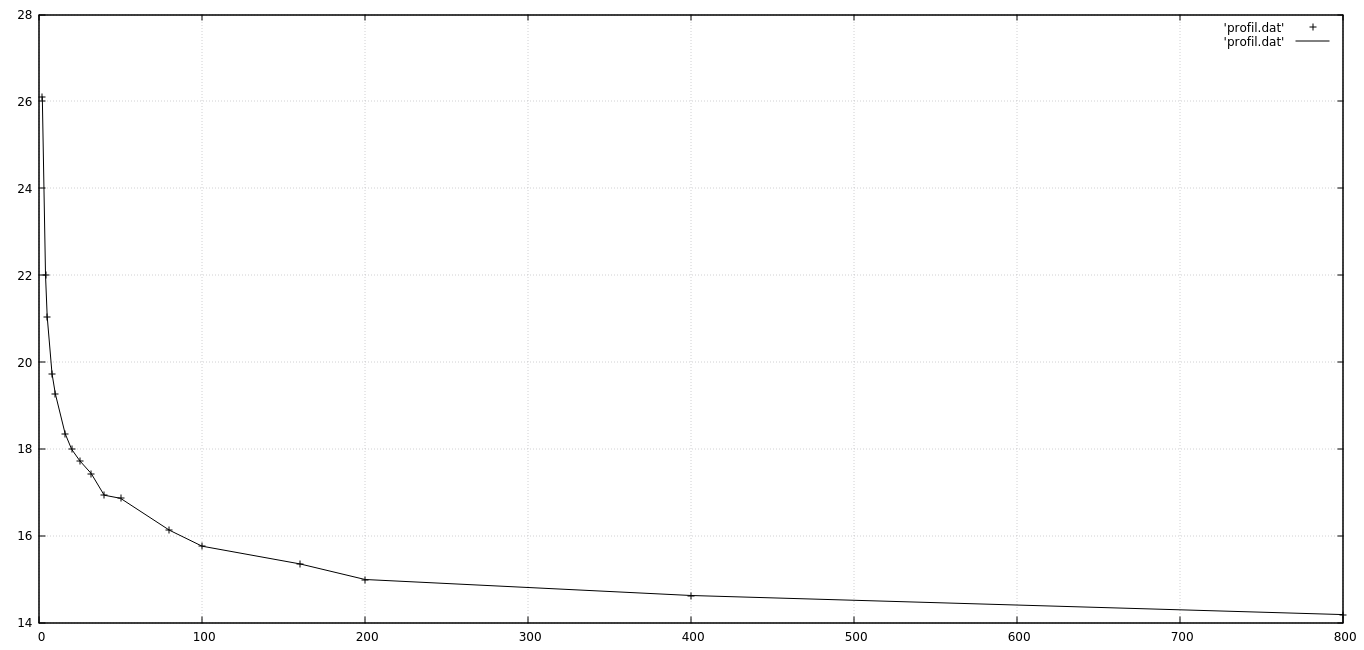
\includegraphics[width=.6\linewidth]{rsc/psnr_ressemblance.png}
                        \end{figure}
                    \end{center}
                \end{block}
            \end{column}

            %----------------------------------
            %-          C3 - LECTURE          -
            %----------------------------------

            \begin{column}{.5\linewidth}
                \setbeamercolor{block title}{fg=white,bg=black} % Colors of the block titles
                \setbeamercolor{block body}{fg=black,bg=white} % Colors of the block titles
                \begin{block}{\centering \textbf{Lecture des pixels}}


                    \begin{center}
                        figure psnr lecture des pixels
                        % \begin{figure}[t]
                        %     
\includegraphics[width=.5\linewidth]{rsc/logo_lirmm.png}
                        % \end{figure}
                    \end{center}
                \end{block}
            \end{column}
        \end{columns}
    \end{frame}
\end{document}
